\documentclass[12pt, a4paper]{article}
\usepackage[utf8]{inputenc}
\usepackage{mathtools}
\usepackage{amsthm}
\usepackage{cancel}
\usepackage{graphicx}
\graphicspath{ {../images/} }

\usepackage{listings}
\usepackage{xcolor}

\usepackage[T1]{fontenc}

\definecolor{codegreen}{rgb}{0,0.6,0}
\definecolor{codegray}{rgb}{0.5,0.5,0.5}
\definecolor{codepurple}{rgb}{0.58,0,0.82}
\definecolor{backcolour}{rgb}{0.95,0.95,0.92}

\lstdefinestyle{mystyle}{
    backgroundcolor=\color{backcolour},   
    commentstyle=\color{codegreen},
    keywordstyle=\color{blue},
    numberstyle=\tiny\color{codegray},
    stringstyle=\color{codegreen},
    basicstyle=\ttfamily\footnotesize,
    breakatwhitespace=false,         
    breaklines=true,                 
    captionpos=b,                    
    keepspaces=true,                 
    numbers=left,                    
    numbersep=5pt,                  
    showspaces=false,                
    showstringspaces=false,
    showtabs=false,                  
    tabsize=2
}

\lstset{style=mystyle}

\title{Obligatorisk oppgave 1, MEK1100, Vår 2021}
\author{Cory Alexander Balaton}
\date{}

\begin{document}

\maketitle 
\newpage



\section*{Oppgave 3}

a)





\section*{Oppgave 4}

a)
\lstinputlisting[language=Python]{../Python/strlin.py}
Koden over gir to plotter: \\
\hspace*{-1.5cm}
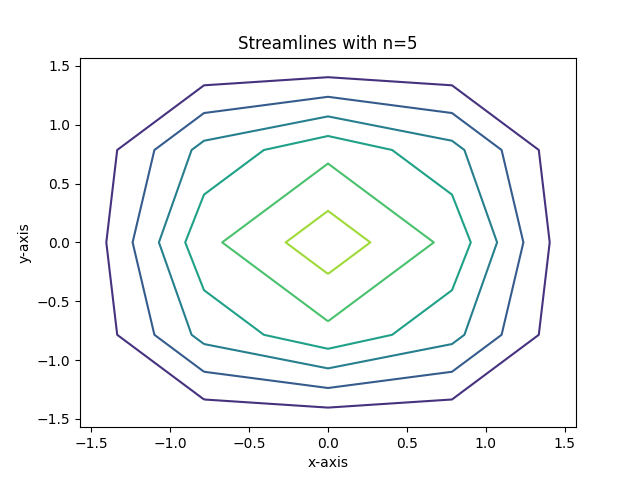
\includegraphics[scale=0.5]{strlin_5}
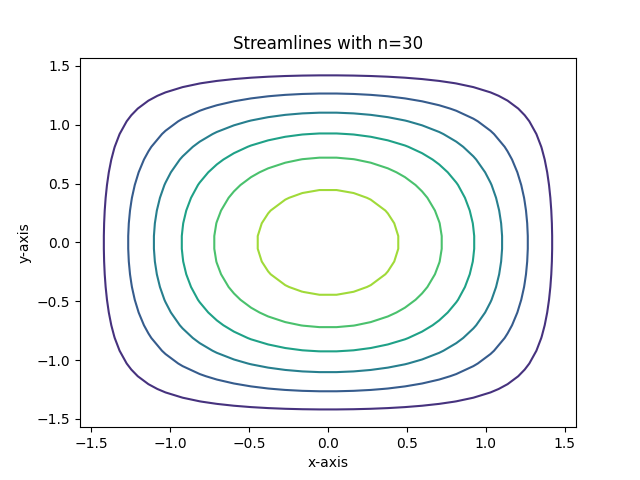
\includegraphics[scale=0.5]{strlin_30}\\

b)
\lstinputlisting[language=Python]{../Python/vec.py}
Koden over gir vektorfeltet under: \\
\hspace*{-1.5cm}
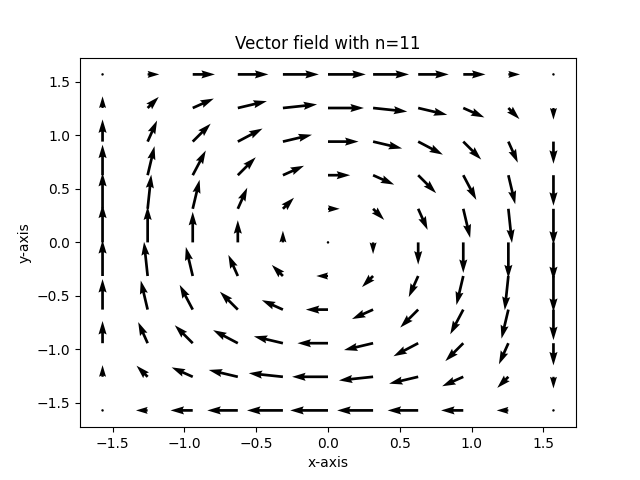
\includegraphics[scale=1]{vec_11.png}


\end{document}